\documentclass[11pt]{article}

\usepackage[margin=1in]{geometry}
\usepackage{graphicx}
\graphicspath{{../artifacts/figures/}{../artifacts/deploys/}}
\usepackage{booktabs}
\usepackage{longtable}
\usepackage{array}
\usepackage{xcolor}
\usepackage{listings}
\usepackage{hyperref}
\usepackage{enumitem}
\usepackage{float}
\usepackage[strings]{underscore}

\hypersetup{
  colorlinks=true,
  linkcolor=blue,
  urlcolor=blue,
  citecolor=blue
}

\setlist[itemize]{leftmargin=1.5em}
\newcommand{\code}[1]{\texttt{#1}}

\lstdefinestyle{codeblock}{
  basicstyle=\ttfamily\small,
  breaklines=true,
  columns=fullflexible,
  frame=single,
  showstringspaces=false,
  backgroundcolor=\color{gray!5}
}
\lstset{style=codeblock}

\title{Complete Fraud Detection Report\\Real-Time Banking Transaction Fraud Detection and Decision Support System}
\author{Repository: \code{Final_Project_DMM501_Group1}}
\date{April 2026}

\begin{document}
\maketitle
\tableofcontents
\newpage

\section{Executive Summary}
This project implements a fraud detection system that combines machine learning inference with operational decision support for transaction handling. The implemented system accepts a transaction feature vector through a FastAPI service, computes an uncalibrated \code{risk_score}, maps that score to a \code{risk_tier} and \code{decision_recommendation}, and creates an \code{alert} and \code{case} for suspicious transactions. The broader system also includes an analyst-facing frontend, case lifecycle management, Prometheus metrics, Grafana dashboards, MLflow runtime tracking, automated tests, and Docker-based deployment components.

The key capability is not only fraud scoring, but the conversion of model output into actionable workflow states. In the implemented design, the machine learning layer acts as a ranking mechanism, while operational services determine whether a transaction should be allowed, sent for manual review, challenged through step-up authentication, held, or blocked. This architecture supports analyst triage, queue management, and investigation tracking rather than treating model output as a final adjudication.

The business objective is to reduce fraud loss, control review workload, and limit unnecessary customer friction. It does so by separating low-risk transactions from review-queue transactions and high-risk transactions, while preserving traceability through \code{alert}, \code{case}, and timeline records. The implementation is strongest as a local, end-to-end fraud decision-support demonstration and MLOps reference system, rather than as a production-grade banking control stack.

\section{Introduction}
Fraud detection remains a central operational problem in banking because digital transactions are high volume, time sensitive, and exposed to multiple attack patterns, including unauthorized card use, account takeover, mule activity, and anomalous transfer behavior. Financial institutions must detect suspicious activity quickly enough to contain loss, while also avoiding unnecessary interruption to legitimate customers.

Traditional rule-based fraud systems remain useful, but they have well-known limitations. Static rules can be brittle, generate excessive false positives, and require substantial manual maintenance as fraud patterns evolve. Rules are also difficult to optimize when risk depends on interactions among many variables rather than a small number of predefined conditions.

Machine learning is therefore useful because it can rank transactions by relative suspiciousness from historical patterns. However, in banking operations, model output alone is insufficient. A practical fraud detection system must integrate scoring with policy decisions, analyst queues, case handling, monitoring, and auditability. This repository reflects that broader framing by combining a supervised fraud model with decision logic, \code{alert} generation, \code{case} workflow, and operational interfaces.

\section{Problem Definition}
The core analytical problem is transaction fraud detection on a highly imbalanced dataset. The repository uses the Kaggle credit card fraud dataset, where fraudulent transactions represent a very small minority of all observations. In such settings, standard accuracy is not meaningful because a naive model can predict the majority class and still appear strong.

The operational problem is more complex than binary classification. A false negative can produce direct financial loss, reputational damage, and delayed investigation. A false positive can create customer friction, reduce transaction completion, and overload analysts with low-value investigations. For this reason, the implemented system converts model output into \code{risk_tier} values and downstream \code{decision_recommendation} values rather than returning only a class label.

The project therefore addresses a decision-support problem: rank transactions by risk, separate suspicious from non-suspicious activity, allocate review capacity using explicit thresholds, and support investigation through \code{alert} and \code{case} management.

\section{Business Context}
Banking fraud controls operate under competing constraints. First, fraud loss matters because delayed intervention can allow rapid cash-out or repeated unauthorized transactions. Second, customer friction matters because unnecessary holds, blocks, or manual reviews can cause legitimate payment failure and dissatisfaction. Third, analyst workload matters because review teams have limited capacity and cannot investigate every transaction manually.

The implemented threshold policy in this repository reflects those constraints. Thresholds are selected using a top-K review-rate policy rather than a single generic cutoff. This means the system is designed to approximate operational review capacity by flagging only the highest-scoring fraction of transactions for review and a smaller fraction for high-risk handling.

The project also acknowledges operational realities beyond scoring. A suspicious transaction must enter an \code{alert} queue, become a \code{case}, move through status transitions, and eventually reach a resolution such as \code{CONFIRMED_FRAUD} or \code{FALSE_POSITIVE}. Monitoring must then track queue size, status transitions, and false-positive outcomes.

\section{System Overview}
The implemented system follows the pipeline below:

\begin{center}
Transaction $\rightarrow$ Validation $\rightarrow$ Feature processing $\rightarrow$ Risk scoring $\rightarrow$ Decision policy $\rightarrow$ Alert generation $\rightarrow$ Case creation $\rightarrow$ Investigation $\rightarrow$ Resolution
\end{center}

\begin{enumerate}[leftmargin=1.5em]
  \item Transaction intake through \code{features} or \code{features_by_name}, with optional \code{transaction_id}, \code{timestamp}, \code{amount}, \code{channel}, and \code{metadata}.
  \item Validation of schema consistency, numeric finiteness, and feature length against model metadata.
  \item Feature processing for inference.
  \item Risk scoring through the deployed model to obtain an uncalibrated \code{risk_score}.
  \item Decision policy mapping to \code{risk_tier} and \code{decision_recommendation}.
  \item Reason-code generation through a heuristic decision-support layer.
  \item \code{Alert} and \code{case} creation for \code{REVIEW} and \code{HIGH} outcomes.
  \item Analyst investigation through queue, case detail, status changes, and timeline.
  \item Resolution through final case outcomes.
\end{enumerate}

\section{Dataset Description}
The repository uses the Kaggle credit card fraud dataset stored locally as \code{data/archive/creditcard.csv} and \code{data/raw/creditcard.csv}. According to the generated repository artifacts, the dataset contains 284{,}807 rows and 31 columns, consisting of \code{Time}, anonymized variables \code{V1} through \code{V28}, \code{Amount}, and the target variable \code{Class}.

Fraud is extremely rare in the data. The generated class distribution report shows 492 fraud records and 284{,}315 non-fraud records, giving a fraud ratio of 0.001727485630620034, or approximately 0.17\%.

The feature set has important limitations for banking interpretation. Most predictors are PCA-transformed variables rather than business-readable fields such as merchant category, destination account, device reputation, customer tenure, or beneficiary risk.

\subsection{Dataset figures}
\begin{figure}[H]
\centering
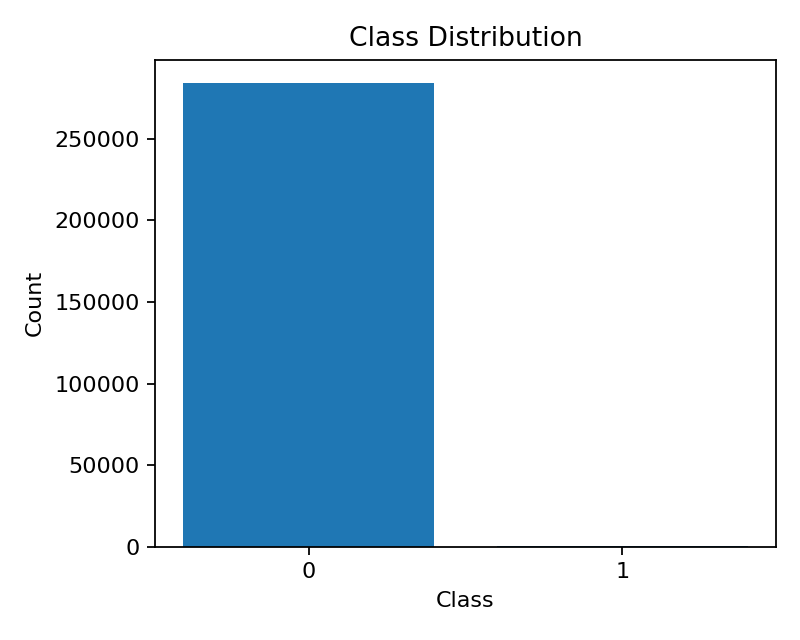
\includegraphics[width=0.78\textwidth]{class_distribution.png}
\caption{Class imbalance in the benchmark dataset (fraud vs non-fraud).}
\end{figure}

\begin{figure}[H]
\centering
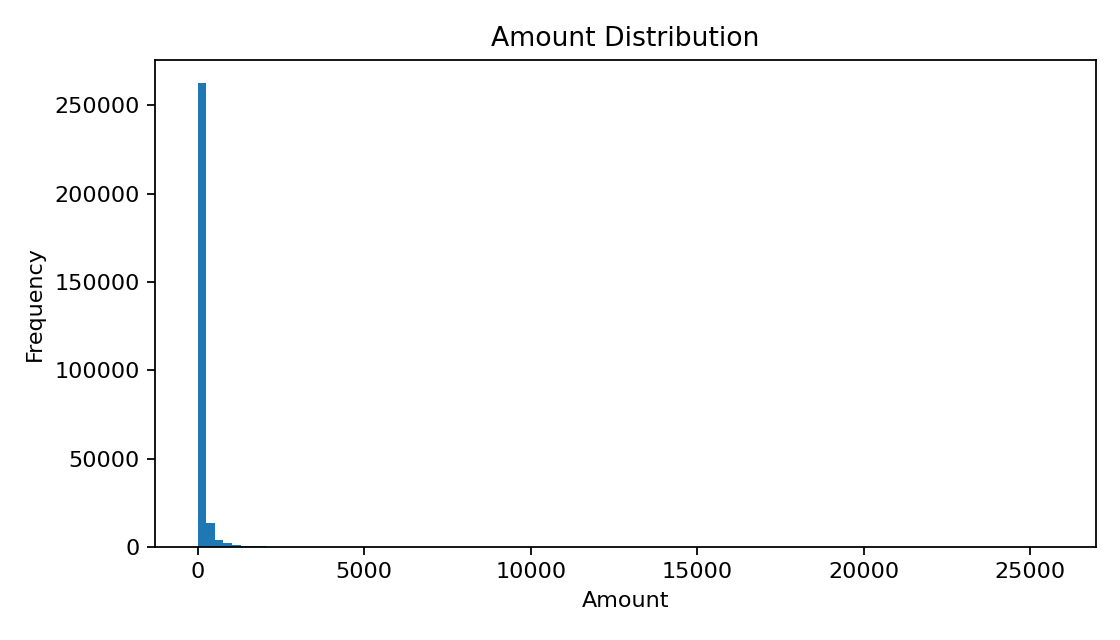
\includegraphics[width=0.95\textwidth]{amount_distribution.png}
\caption{Transaction amount distribution.}
\end{figure}

\begin{figure}[H]
\centering
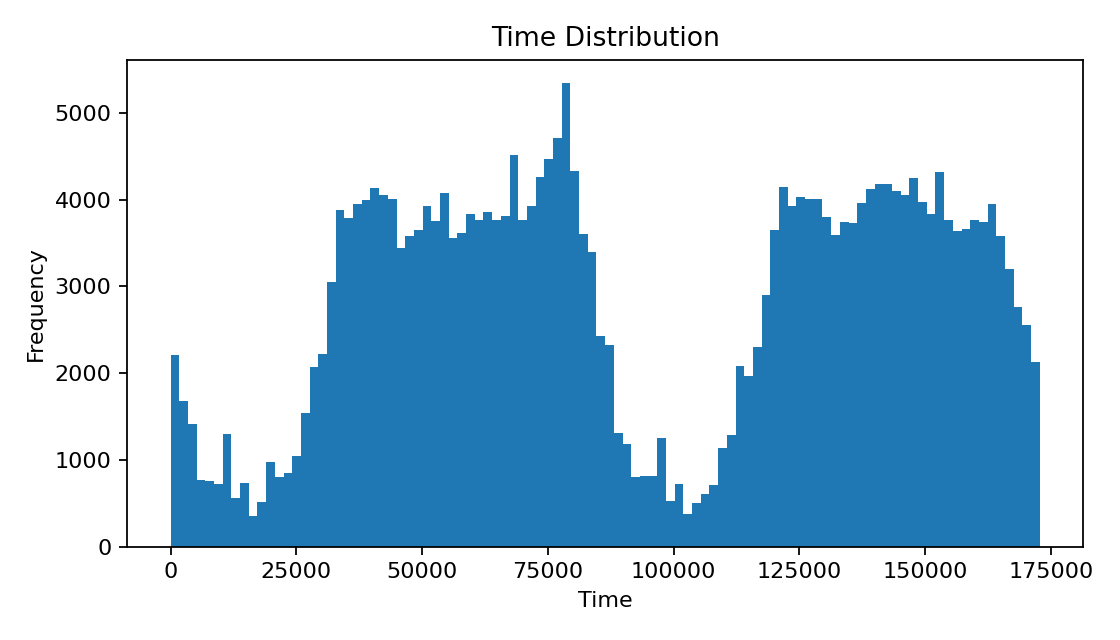
\includegraphics[width=0.95\textwidth]{time_distribution.png}
\caption{Transaction time distribution.}
\end{figure}

\section{Data Challenges}
The first data challenge is extreme class imbalance. Because fraud is rare, a classifier can produce deceptively strong aggregate metrics while still missing many fraudulent transactions or generating too many false alerts. This is why the repository emphasizes PR-AUC, threshold tuning, and operating-point metrics instead of generic accuracy.

The second challenge is interpretability. The PCA-style \code{V1}--\code{V28} variables are mathematically useful but operationally opaque. The implemented reason codes therefore rely partly on policy thresholds and optional metadata heuristics rather than on inherently interpretable core features.

The third challenge is simulation realism. Although the project is framed as a banking fraud detection system, the underlying dataset does not contain the full operational context of a bank.

\section{Machine Learning Pipeline}
The repository contains an explicit training and model-selection workflow in \code{src/pipelines/run_model_workflow.py} and \code{src/pipelines/train_pipeline.py}. The workflow reads the credit card dataset, performs exploratory checks and schema validation, splits data into train, validation, and test subsets, and benchmarks multiple models.

The implemented workflow includes preprocessing, model training, evaluation, threshold tuning, and artifact saving. The saved deployment artifact identifies the selected model as a logistic regression pipeline. The threshold policy is explicitly documented in \code{artifacts/models/model_info.json} as a capacity-driven top-K approach with \code{review_top_rate=0.01} and \code{high_top_rate=0.002}.

\section{Model Evaluation}
For fraud detection, PR-AUC is more informative than ROC-AUC because the positive class is extremely rare. ROC-AUC can remain high even when a model produces many false positives at the operating point that matters to analysts. PR-AUC focuses more directly on the precision-recall trade-off under class imbalance.

\subsection{Model comparison}
\begin{table}[H]
\centering
\begin{tabular}{lrrrrrrl}
\toprule
Model & Threshold & Precision & Recall & F1 & ROC-AUC & PR-AUC & Status \\
\midrule
Logistic Regression (Review) & 0.7391 & 0.1470 & 0.8510 & 0.2510 & 0.9684 & 0.6300 & Selected in deployed artifacts \\
LightGBM (Review) & 0.0000004 & 0.1330 & 0.7700 & 0.2270 & 0.9288 & 0.6290 & Benchmarked candidate \\
\bottomrule
\end{tabular}
\caption{Validation operating-point comparison from repository benchmark artifacts.}
\end{table}

The repository also stores the final deployed evaluation metrics at the operating thresholds used for decision support. At the review threshold, precision is 0.1462 and recall is 0.8514. At the high threshold, precision is 0.8429 and recall is 0.7973. These figures show the trade-off between broader queue capture at the review threshold and tighter containment at the high threshold.

\subsection{Model evaluation figures}
\begin{figure}[H]
\centering
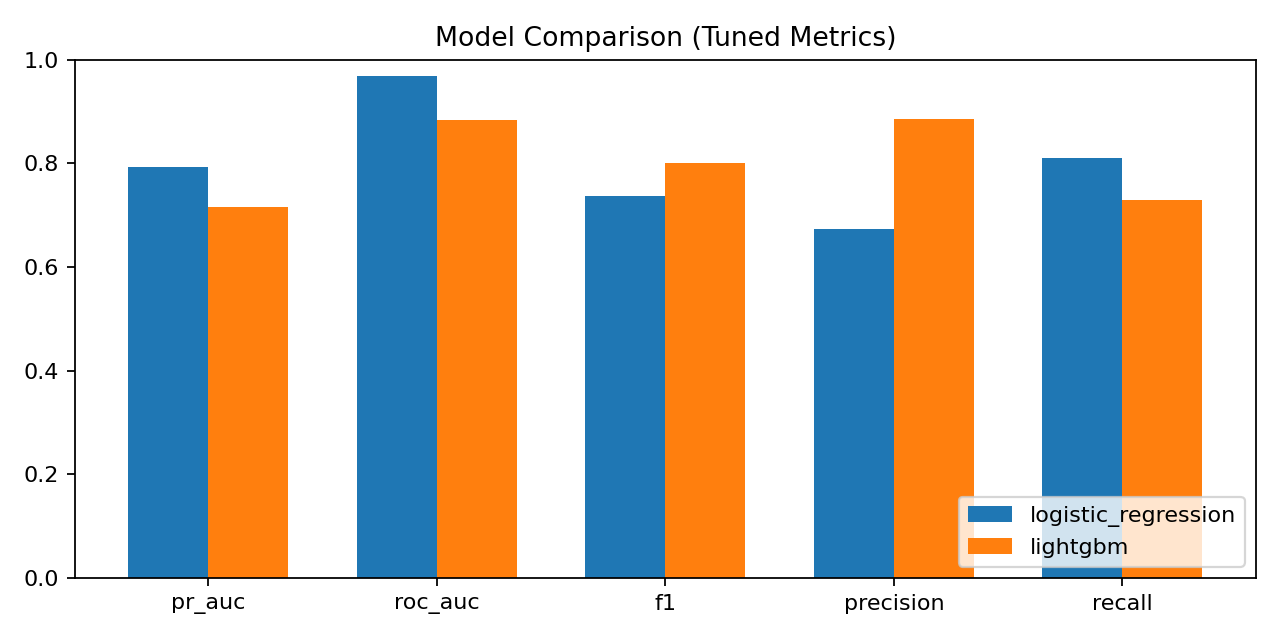
\includegraphics[width=0.95\textwidth]{model_comparison.png}
\caption{Model benchmark comparison summary from saved artifacts.}
\end{figure}

\begin{figure}[H]
\centering
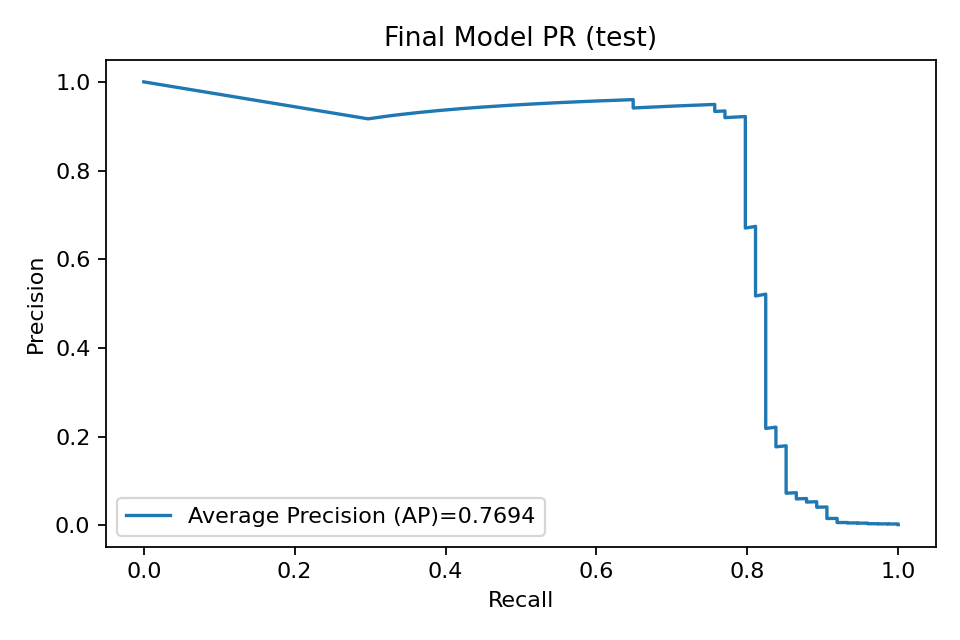
\includegraphics[width=0.49\textwidth]{final_pr_curve.png}
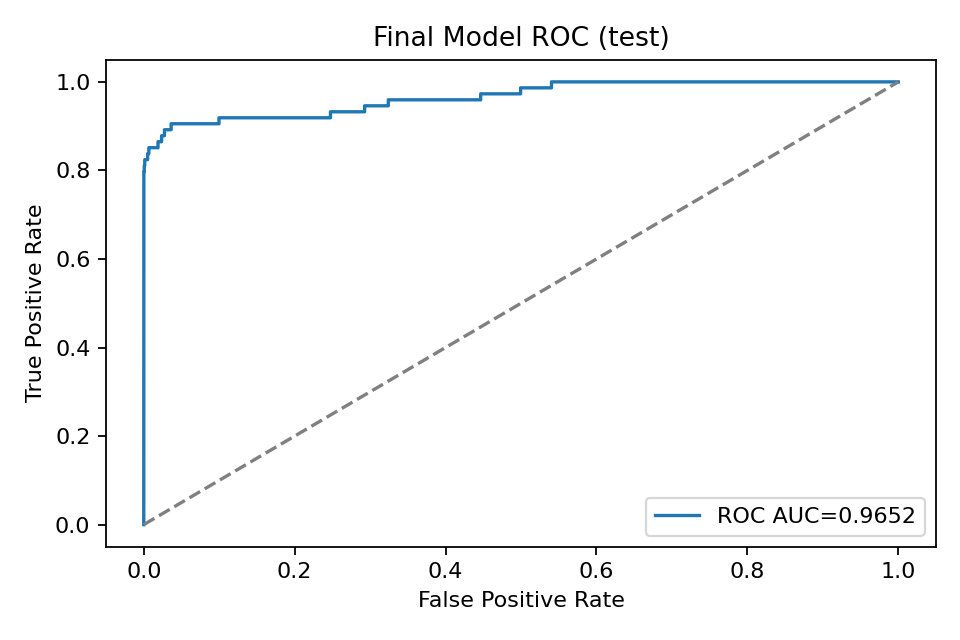
\includegraphics[width=0.49\textwidth]{final_roc_curve.png}
\caption{Final deployed model PR curve (left) and ROC curve (right).}
\end{figure}

\begin{figure}[H]
\centering
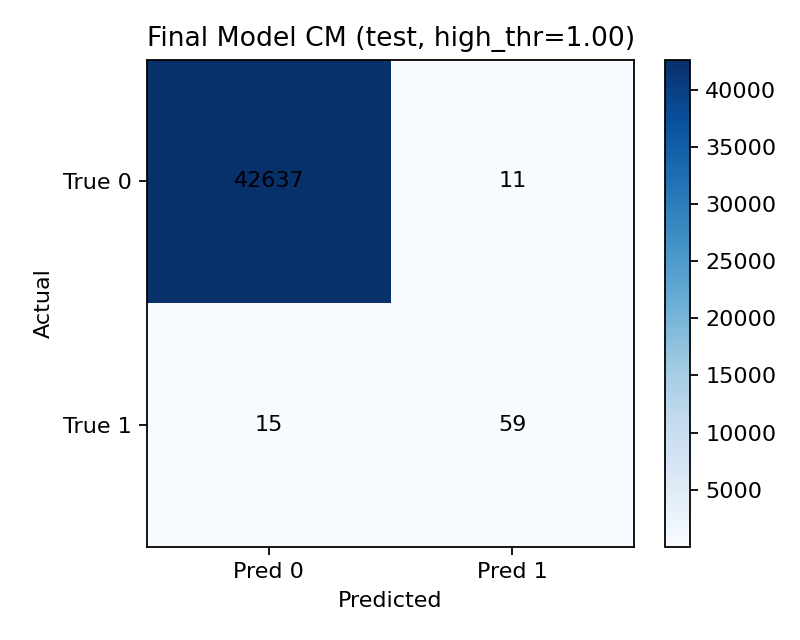
\includegraphics[width=0.78\textwidth]{final_confusion_matrix.png}
\caption{Final deployed model confusion matrix at the selected operating point.}
\end{figure}

\begin{figure}[H]
\centering
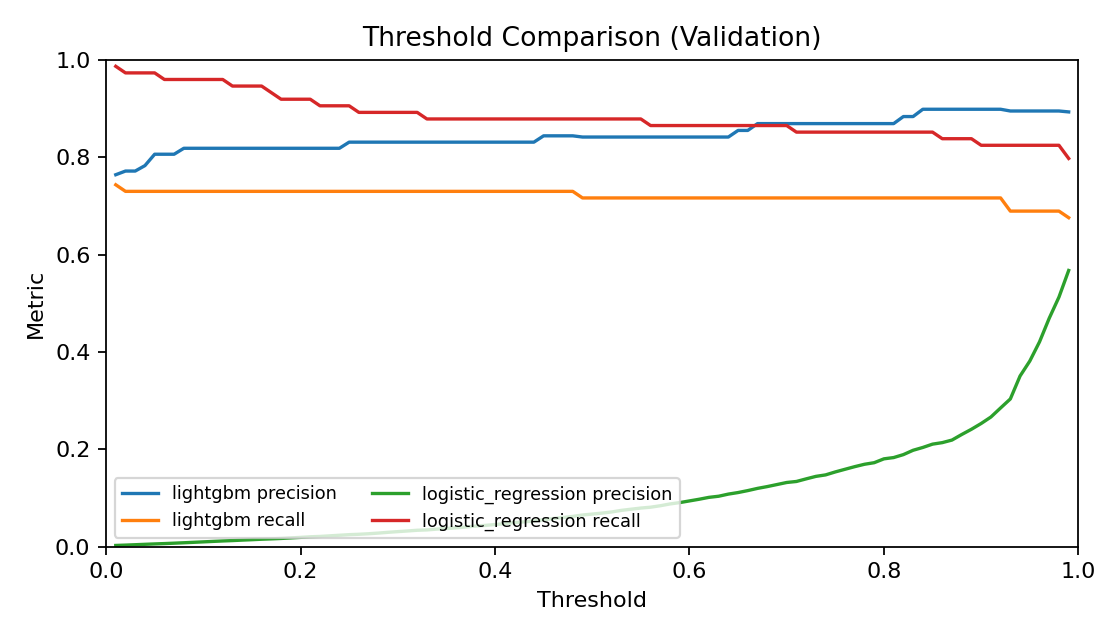
\includegraphics[width=0.95\textwidth]{threshold_comparison.png}
\caption{Threshold comparison evidence supporting review/high policy tiers.}
\end{figure}

\begin{figure}[H]
\centering
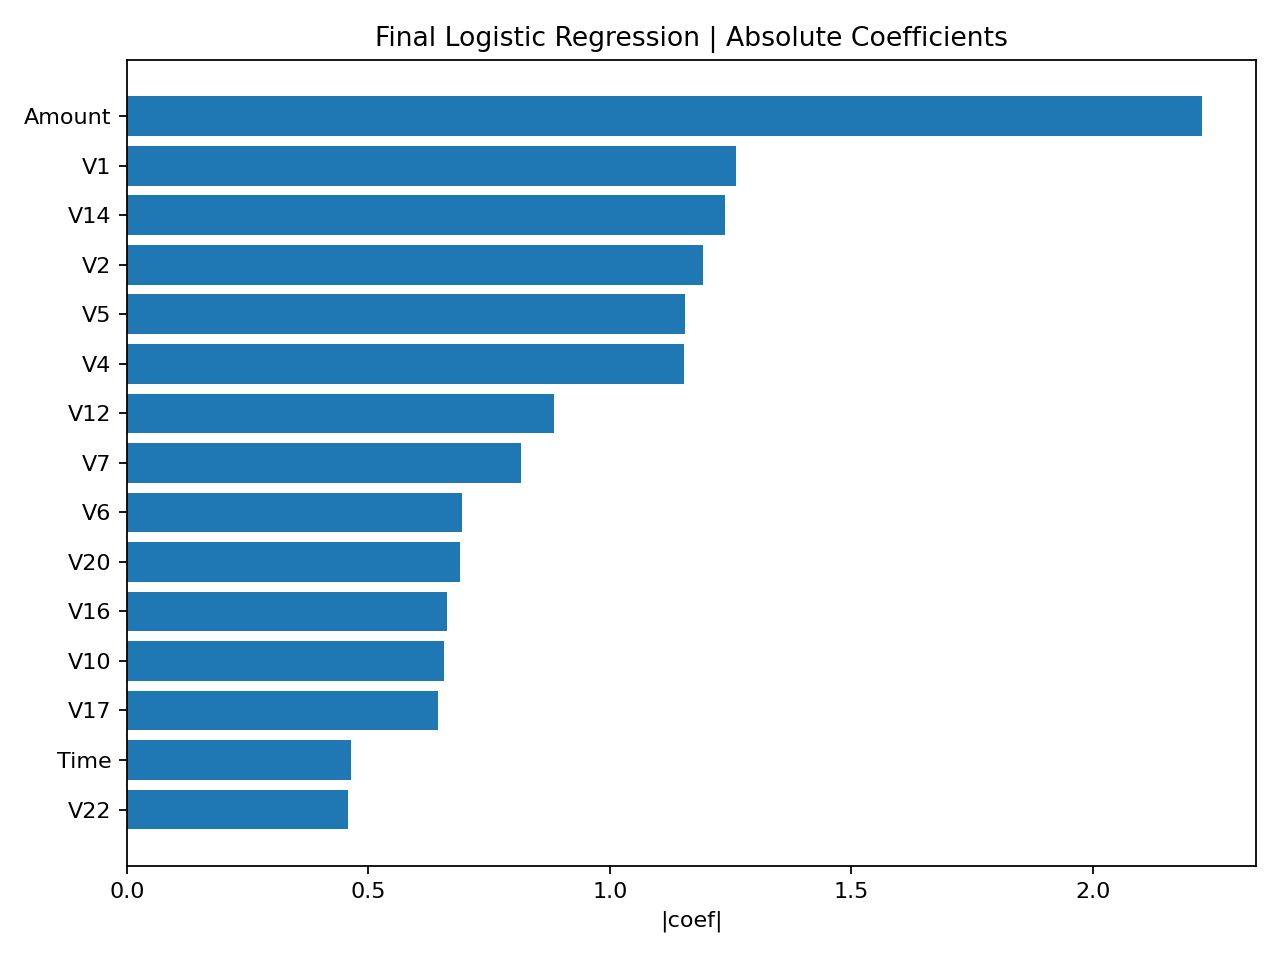
\includegraphics[width=0.95\textwidth]{final_feature_importance.png}
\caption{Feature importance evidence from saved artifacts (model-dependent).}
\end{figure}

\begin{figure}[H]
\centering
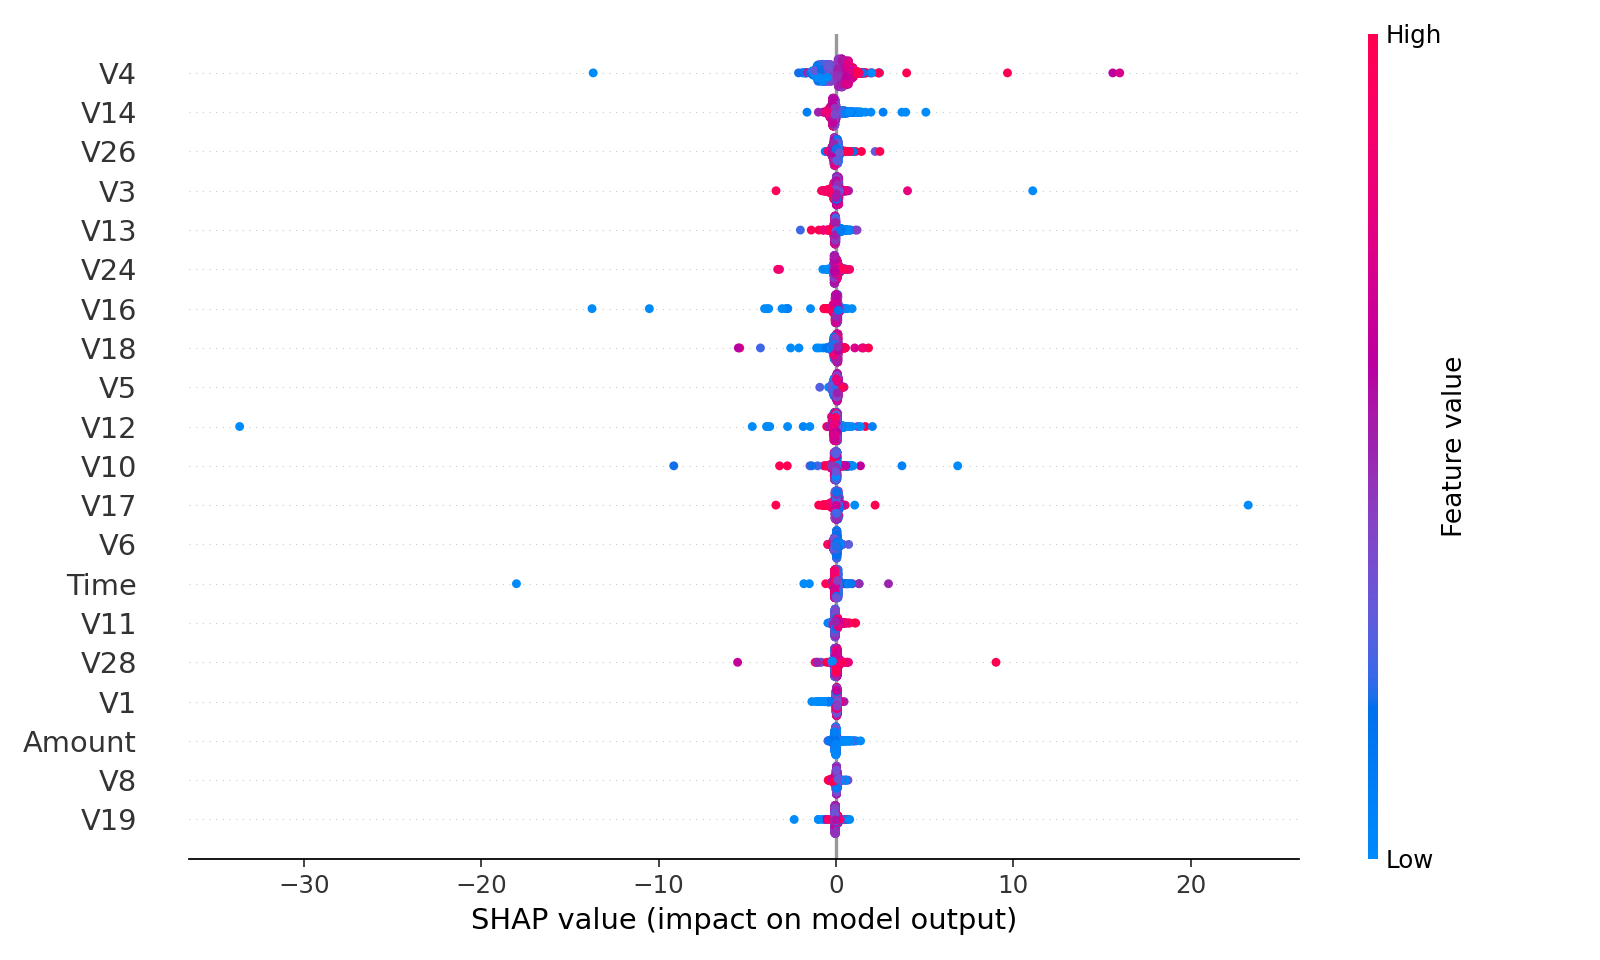
\includegraphics[width=0.95\textwidth]{shap_summary.png}
\caption{SHAP summary plot from saved artifacts (interpretation aid; not causal proof).}
\end{figure}

\section{Risk Scoring and Decision Logic}
The API exposes \code{risk_score} in the range \([0,1]\), but this score is explicitly described in the repository as uncalibrated. It should therefore be interpreted as a ranking signal rather than a calibrated fraud probability.

The deployed thresholds are:
\begin{itemize}
  \item review threshold: \code{0.7391262534904803}
  \item high-risk threshold: \code{0.9999047447184487}
\end{itemize}

The implemented \code{risk_tier} logic is:
\begin{itemize}
  \item \code{LOW} if \code{risk_score < threshold_review}
  \item \code{REVIEW} if \code{threshold_review <= risk_score < threshold_high}
  \item \code{HIGH} if \code{risk_score >= threshold_high}
\end{itemize}

The implemented \code{decision_recommendation} logic is:
\begin{itemize}
  \item \code{ALLOW} for \code{LOW}
  \item \code{STEP_UP_AUTH} for digital-channel \code{REVIEW}
  \item \code{MANUAL_REVIEW} for non-digital-channel \code{REVIEW}
  \item \code{HOLD} for default \code{HIGH}
  \item \code{BLOCK} for \code{HIGH} when amount is at least 1500.0
\end{itemize}

\begin{table}[H]
\centering
\begin{tabular}{lll}
\toprule
Score condition & \code{risk_tier} & \code{decision_recommendation} \\
\midrule
\code{< threshold_review} & \code{LOW} & \code{ALLOW} \\
\code{>= threshold_review} and \code{< threshold_high} & \code{REVIEW} & \code{STEP_UP_AUTH} or \code{MANUAL_REVIEW} \\
\code{>= threshold_high} & \code{HIGH} & \code{HOLD} or \code{BLOCK} \\
\bottomrule
\end{tabular}
\caption{Score-to-decision mapping.}
\end{table}

\section{Fraud Detection Workflow}
The implemented fraud detection workflow is as follows:
\begin{enumerate}[leftmargin=1.5em]
  \item A transaction arrives through \code{POST /predict}.
  \item The backend validates the request and extracts the feature vector.
  \item The scoring service computes the uncalibrated \code{risk_score}.
  \item The decision service assigns a \code{risk_tier} and \code{decision_recommendation}.
  \item The reason-code service generates decision-support cues.
  \item If the result is \code{REVIEW} or \code{HIGH}, the case service creates an \code{alert} and linked \code{case}.
  \item The transaction enters the fraud alert queue exposed by \code{GET /alerts} and \code{GET /cases}.
  \item An analyst can move the \code{case} into \code{IN_REVIEW}, investigate it, update status, and resolve the outcome.
  \item Timeline events record the sequence from scoring to closure.
\end{enumerate}

The implemented \code{case} lifecycle statuses are \code{NEW}, \code{QUEUED}, \code{IN_REVIEW}, \code{ESCALATED}, \code{CONFIRMED_FRAUD}, \code{FALSE_POSITIVE}, \code{BLOCKED}, \code{RELEASED}, and \code{RESOLVED}. Timeline events include \code{TRANSACTION_RECEIVED}, \code{RISK_SCORED}, \code{FLAGGED}, \code{ALERT_CREATED}, \code{CASE_ASSIGNED}, \code{INVESTIGATION_STARTED}, resolution events, and \code{CASE_CLOSED}.

\begin{table}[H]
\centering
\begin{tabular}{p{0.2\linewidth}p{0.45\linewidth}p{0.23\linewidth}}
\toprule
Stage & Implemented behavior & Output \\
\midrule
Transaction intake & API accepts features and optional transaction context & Validated request \\
Risk scoring & Model computes uncalibrated \code{risk_score} & Score in \([0,1]\) \\
Decision policy & Score mapped to \code{risk_tier} and \code{decision_recommendation} & Operational action guidance \\
Alert creation & \code{REVIEW} and \code{HIGH} create \code{alert} and \code{case} & Queue item \\
Investigation & Analyst updates status and reviews reason codes and timeline & Ongoing \code{case} \\
Resolution & Analyst marks confirmed fraud, false positive, blocked, released, or resolved & Closed outcome \\
\bottomrule
\end{tabular}
\caption{Fraud workflow summary.}
\end{table}

\section{Backend System Design}
The backend is implemented as a FastAPI application. It loads the trained model at startup, instantiates a stream simulator when a model is available, and constructs a case repository through an environment-driven repository factory.

The key backend services are the scoring service, decision service, reason code service, and case service. The core scoring endpoint is \code{POST /predict}. Supporting endpoints include health, metrics, stream simulation, feature schema access, dataset sampling, alert retrieval, case retrieval, status updates, case resolution, and timeline retrieval.

\subsection{Core request flow: \code{POST /predict}}
At a high level, the backend converts a prediction request into operational outputs through the following deterministic sequence.

\begin{lstlisting}[language=Python]
request -> validate schema + auth + rate limit
       -> resolve features (features OR features_by_name)
       -> validate feature vector length and numeric finiteness
       -> score_transaction(model, features) -> risk_score
       -> decide_risk_action(risk_score, thresholds) -> risk_tier, action, recommendation
       -> generate_reason_codes(...) -> reason_codes + summary
       -> if risk_tier in {REVIEW, HIGH}: create alert + case + timeline events
       -> record Prometheus metrics + audit event
       -> return PredictResponse(...)
\end{lstlisting}

Key implementation references: request handling in \code{src/api/main.py}, scoring in \code{src/services/scoring_service.py}, decision logic in \code{src/services/decision_service.py}, workflow orchestration in \code{src/services/case_service.py}, and persistence in \code{src/repositories/}.

\subsection{API contract evidence}
\begin{figure}[H]
\centering

\includegraphics[width=0.95\textwidth]{swagger-docs.png}
\caption{Swagger/OpenAPI documentation for the FastAPI backend (local deployment evidence screenshot).}
\end{figure}

\subsection{API endpoint table}
\begin{longtable}{p{0.22\linewidth}p{0.1\linewidth}p{0.42\linewidth}p{0.16\linewidth}}
\toprule
Endpoint & Method & Purpose & Status \\
\midrule
\endhead
\code{/health} & GET & API and model metadata, thresholds, queue size, persistence mode & Implemented \\
\code{/features/schema} & GET & Return expected feature contract & Implemented \\
\code{/features/random} & GET & Return demo feature vectors & Implemented \\
\code{/metrics} & GET & Prometheus metrics export & Implemented \\
\code{/predict} & POST & Score transaction and optionally create \code{alert} and \code{case} & Implemented \\
\code{/stream/pull} & GET & Pull pre-scored demo events & Implemented \\
\code{/alerts} & GET & List fraud alerts & Implemented \\
\code{/alerts/\{alert_id\}} & GET & Retrieve alert detail & Implemented \\
\code{/alerts/\{alert_id\}/status} & POST & Update linked case status via alert & Implemented \\
\code{/cases} & GET & List cases & Implemented \\
\code{/cases/\{case_id\}} & GET & Retrieve case detail & Implemented \\
\code{/cases/\{case_id\}/status} & POST & Update case lifecycle status & Implemented \\
\code{/cases/\{case_id\}/resolve} & POST & Resolve case outcome & Implemented \\
\code{/cases/\{case_id\}/timeline} & GET & Retrieve investigation timeline & Implemented \\
\code{/audit/events} & GET & Retrieve audit events & Implemented, ancillary \\
\code{/dataset/samples} & GET & Fetch unlabeled sample rows & Implemented \\
\code{/internal/dataset/samples} & GET & Fetch labeled sample rows with token protection & Implemented, internal \\
\bottomrule
\end{longtable}

For storage, the system supports two repository modes. The in-memory repository is fully implemented and used as the default demo mode. The SQL repository is implemented in code, covered by integration testing, and wired into Docker Compose through PostgreSQL. SQL-backed persistence is configurable and operational when enabled.

\section{Frontend System}
The frontend is an analyst-facing dashboard implemented in static HTML, CSS, and JavaScript. It connects to the backend API, displays model and threshold metadata, supports live streaming views, and provides a review workflow for suspicious transactions.

The implemented frontend includes a dashboard view for live stream control and summary KPIs, a real-time transaction feed, a fraud alert queue, a review view with case filtering and paging, a case detail panel, and case status actions such as \code{IN_REVIEW}, \code{CONFIRMED_FRAUD}, \code{FALSE_POSITIVE}, and resolution actions.

The frontend also displays a clear score semantics cue stating that the score is uncalibrated rather than a true fraud probability. The UI is therefore more than a visualization layer; it acts as the client for analyst operations against the backend's \code{alert} and \code{case} APIs.

\subsection{Frontend figures}
\begin{figure}[H]
\centering
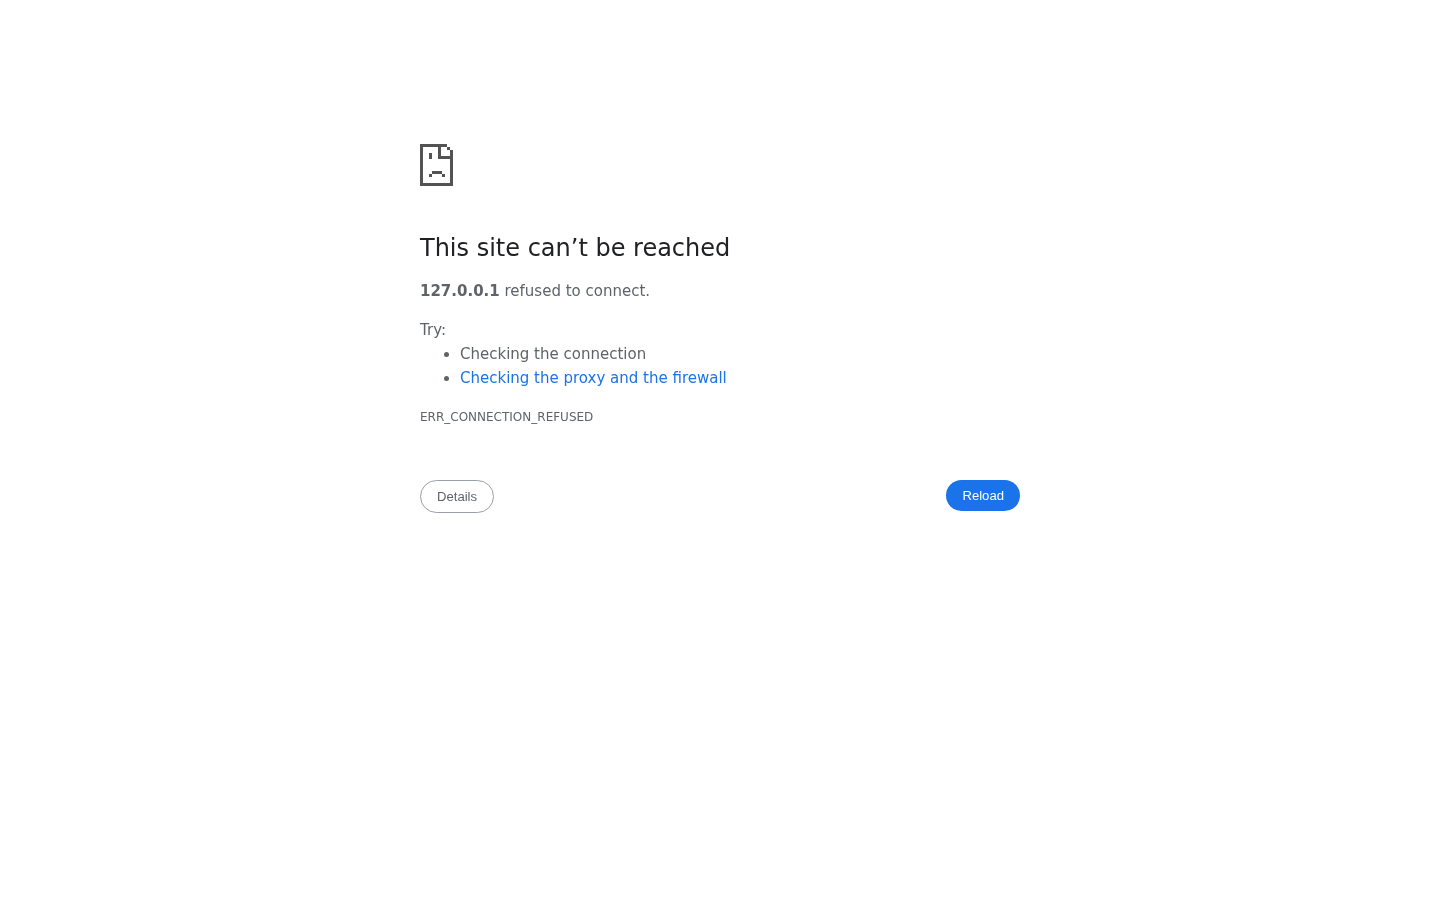
\includegraphics[width=0.95\textwidth]{frontend_dashboard.png}
\caption{Analyst dashboard view (local deployment evidence screenshot).}
\end{figure}

\section{Monitoring and Observability}
The backend exposes Prometheus metrics and includes Grafana dashboard configuration plus MLflow runtime tracking. Monitoring is critical in fraud systems because operational failure can arise from more than model degradation. High latency, queue buildup, false-positive spikes, or unusually low scoring traffic can each undermine fraud operations even when the model artifact itself is unchanged.

The implemented Prometheus metrics include API request volume and status counts, API latency histograms, fraud prediction counts by tier, \code{risk_tier} distribution, \code{decision_recommendation} distribution, \code{alert} and \code{case} creation counts, \code{case} status transition counts, \code{review_queue_size}, confirmed fraud counts, false-positive counts, and risk score aggregates.

The implemented Prometheus alert rules include high 5xx error rate, high p95 API latency, unusually low prediction traffic, unusually high prediction traffic, review queue backlog, and false-positive spike.

MLflow runtime tracking is also implemented. The tracker records runtime traffic metrics such as total requests, predict calls, stream pulls, scored events, average \code{risk_score}, tier totals, HTTP status families, and decision totals.

\subsection{Monitoring figures}
\begin{figure}[H]
\centering
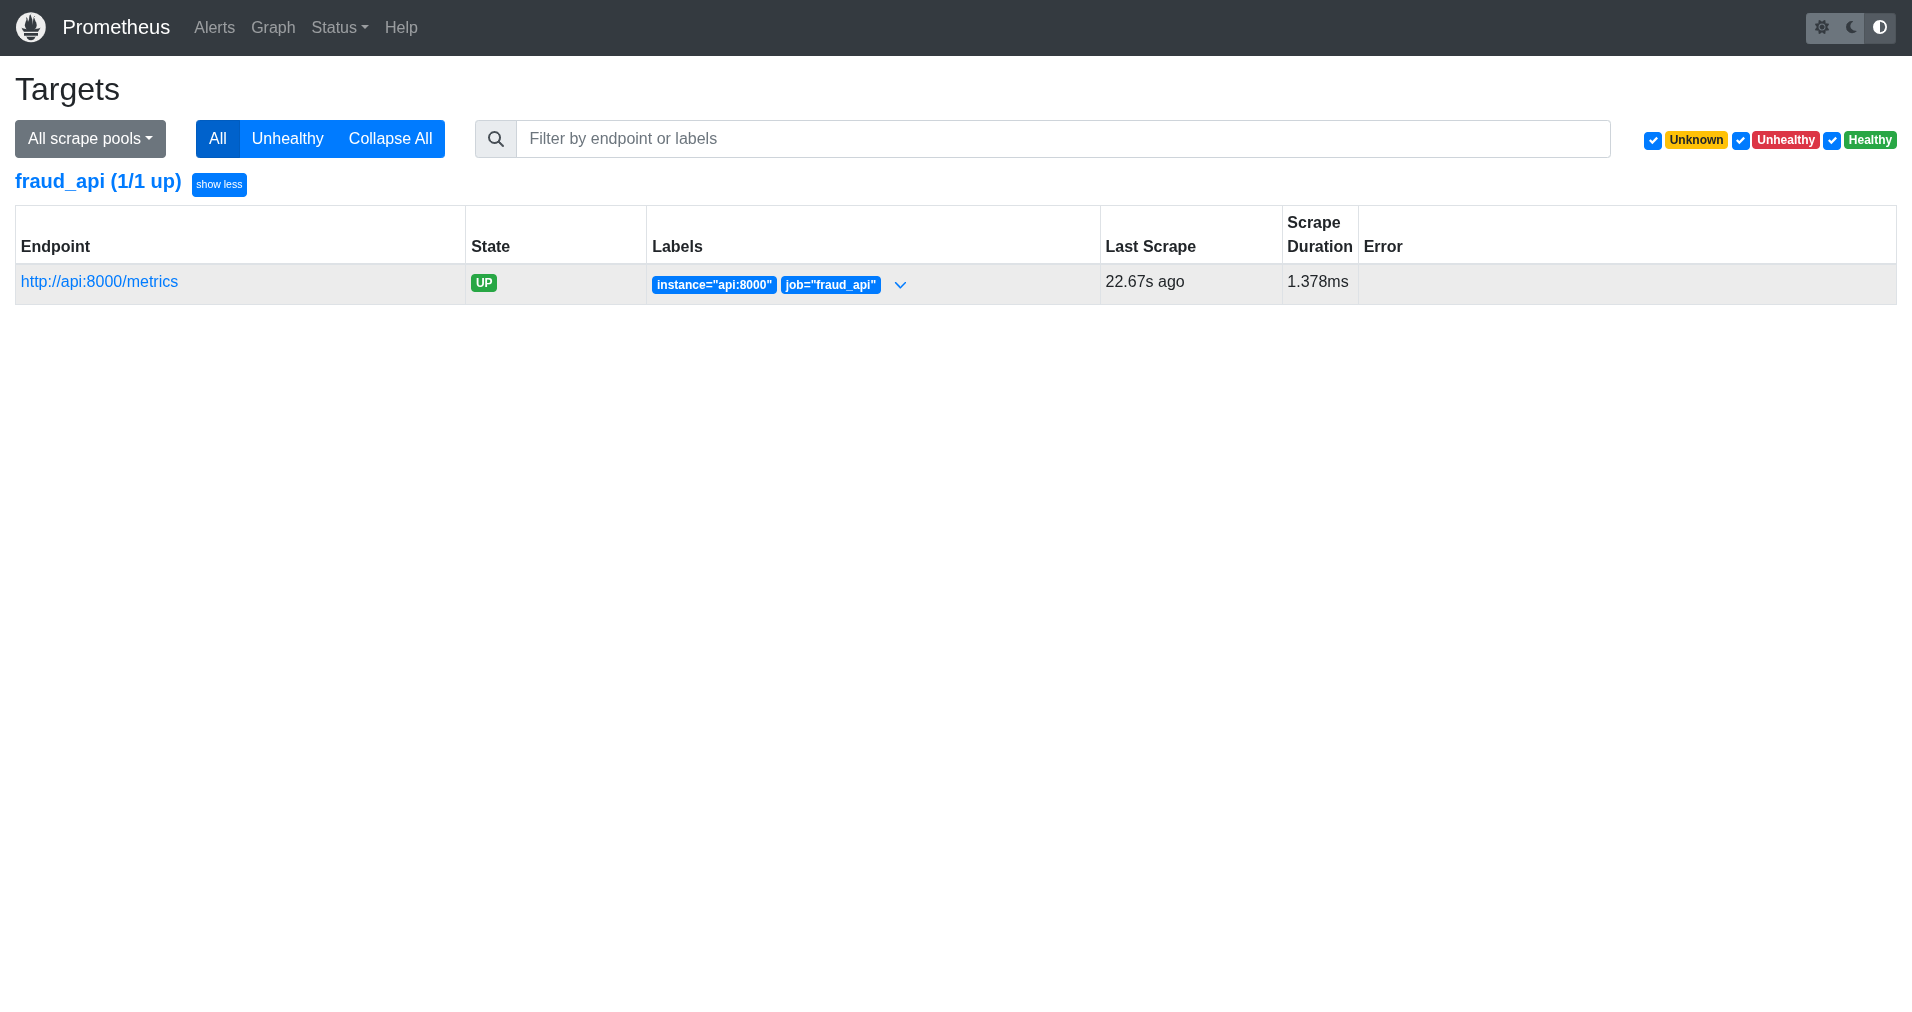
\includegraphics[width=0.95\textwidth]{Prometheus-targets.png}
\caption{Prometheus scrape targets (deployment evidence screenshot).}
\end{figure}

\begin{figure}[H]
\centering
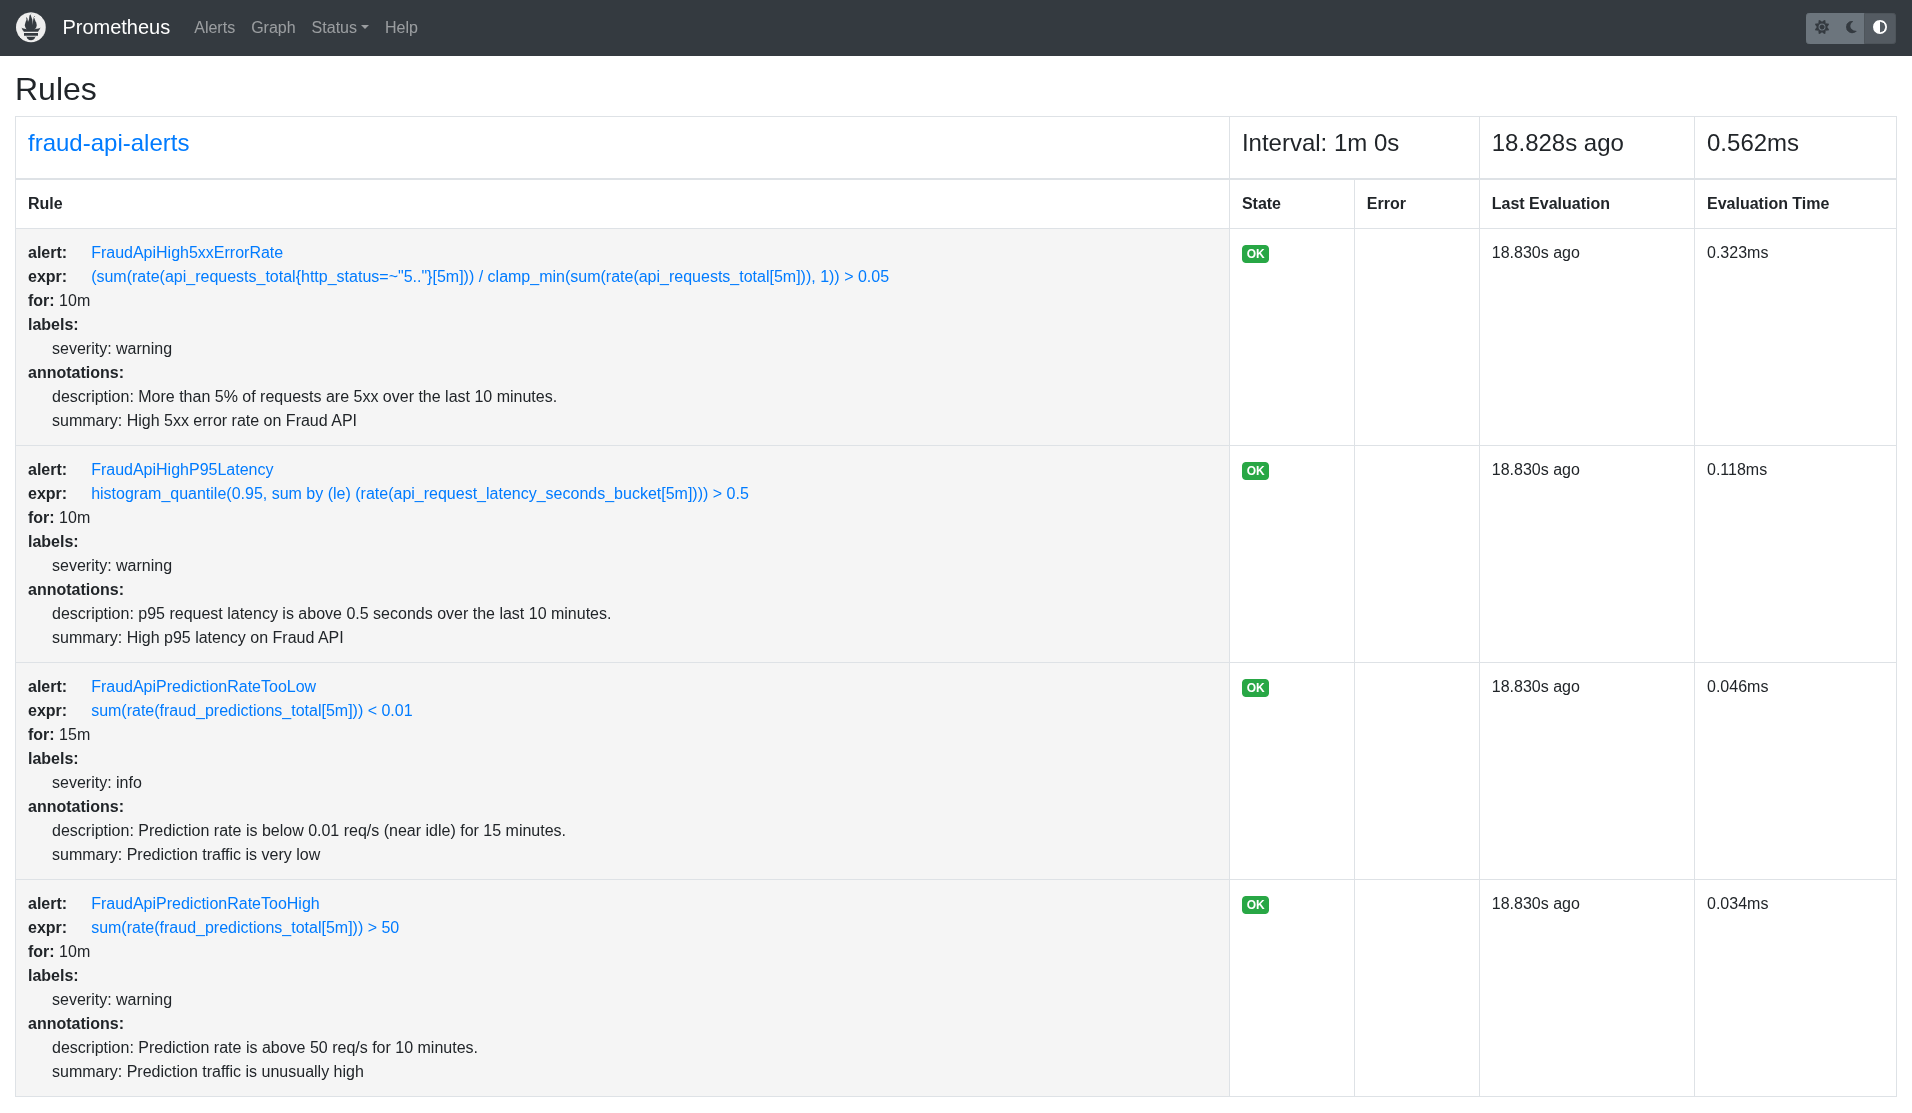
\includegraphics[width=0.95\textwidth]{Prometheus-rules.png}
\caption{Prometheus alert rules loaded and evaluated (deployment evidence screenshot).}
\end{figure}

\begin{figure}[H]
\centering
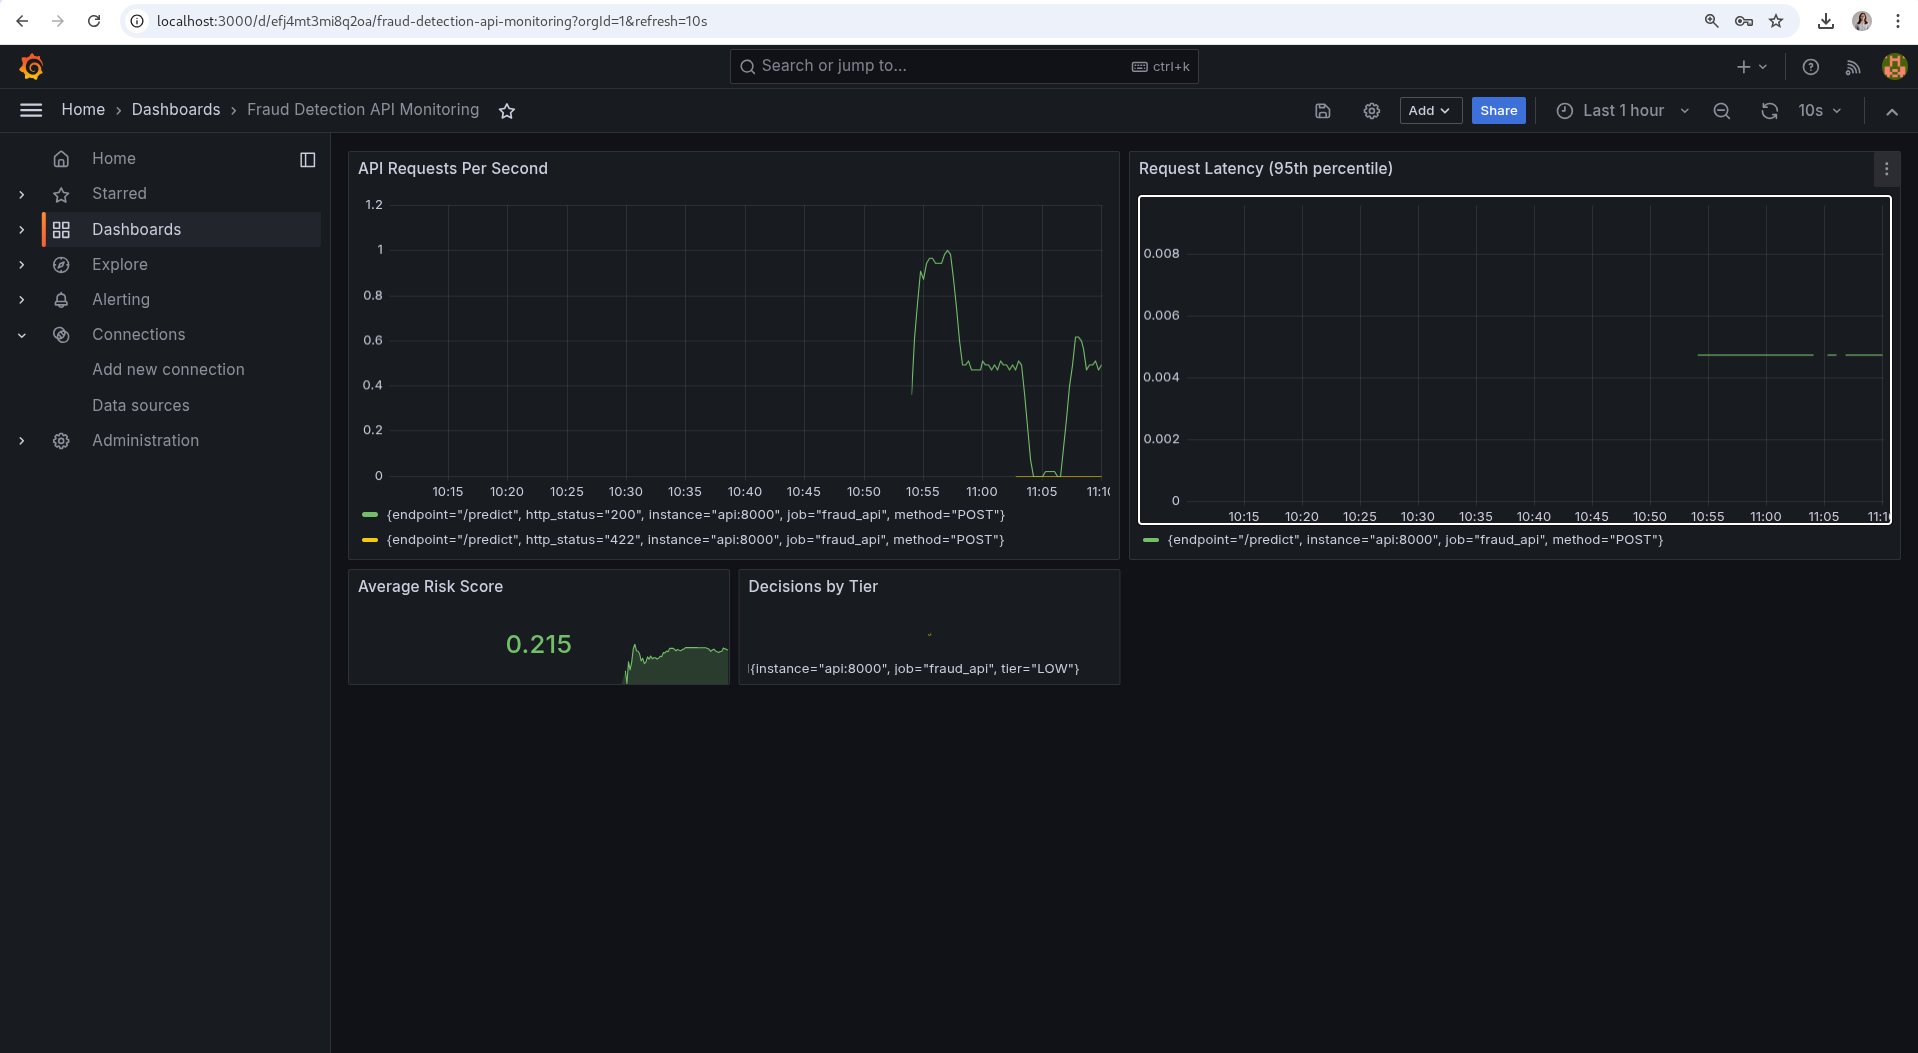
\includegraphics[width=0.95\textwidth]{Grafana-dashboard.png}
\caption{Grafana monitoring dashboard for the fraud API (deployment evidence screenshot).}
\end{figure}

\section{Deployment Architecture}
The repository includes a Docker Compose deployment that orchestrates the broader system end to end. The defined services are API, frontend, Prometheus, Grafana, MLflow, and PostgreSQL.

The API container loads the saved fraud model and mounts the artifacts volume. The frontend container serves the analyst dashboard. Prometheus scrapes the API metrics endpoint and loads alert rules. Grafana reads provisioned dashboards. MLflow hosts experiment and runtime tracking. PostgreSQL provides the durable repository option when the API is configured for SQL persistence.

\subsection{Docker Compose topology (evidence)}
\begin{figure}[H]
\centering
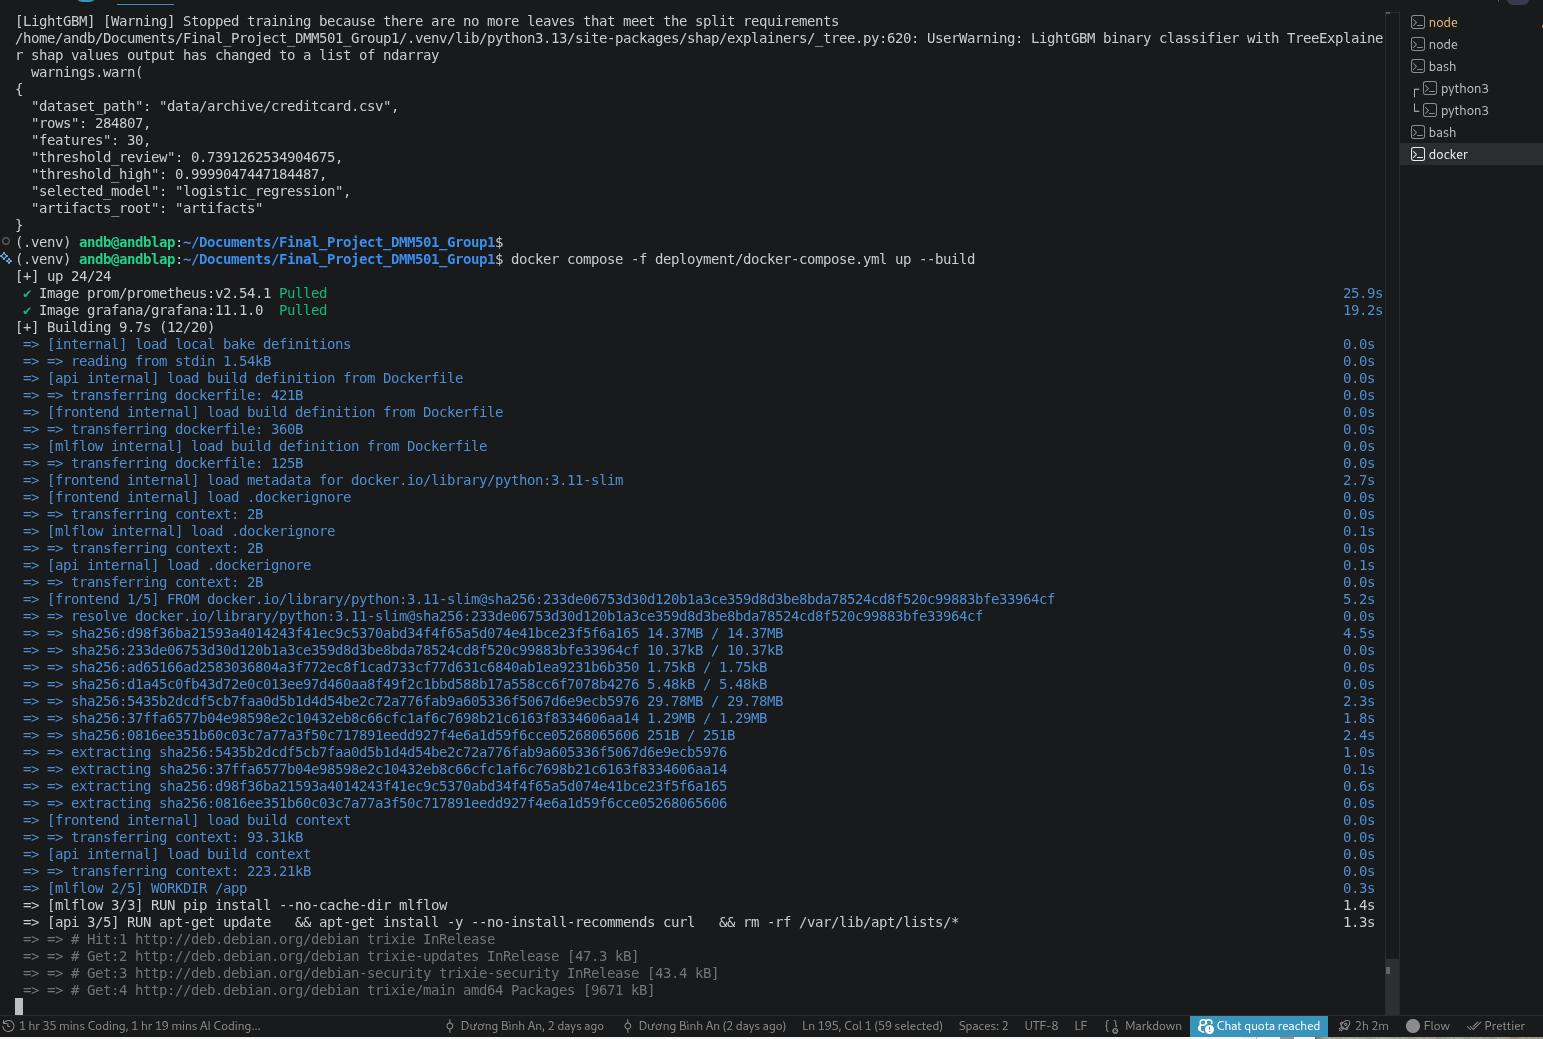
\includegraphics[width=0.95\textwidth]{docker-compose.png}
\caption{Docker Compose topology screenshot (deployment evidence).}
\end{figure}

\subsection{Local deployment steps}
The recommended demo deployment path is Docker Compose:

\begin{lstlisting}[language=bash]
# From repo root:
docker compose -f deployment/docker-compose.yml up --build
\end{lstlisting}

Key service URLs (default ports):
\begin{itemize}
  \item API docs: \code{http://localhost:8000/docs}
  \item Frontend: \code{http://localhost:8082/}
  \item Prometheus: \code{http://localhost:9090/}
  \item Grafana: \code{http://localhost:3000/} (admin password configured by \code{GF\_SECURITY\_ADMIN\_PASSWORD})
  \item MLflow: \code{http://localhost:5000/}
\end{itemize}

\begin{figure}[H]
\centering
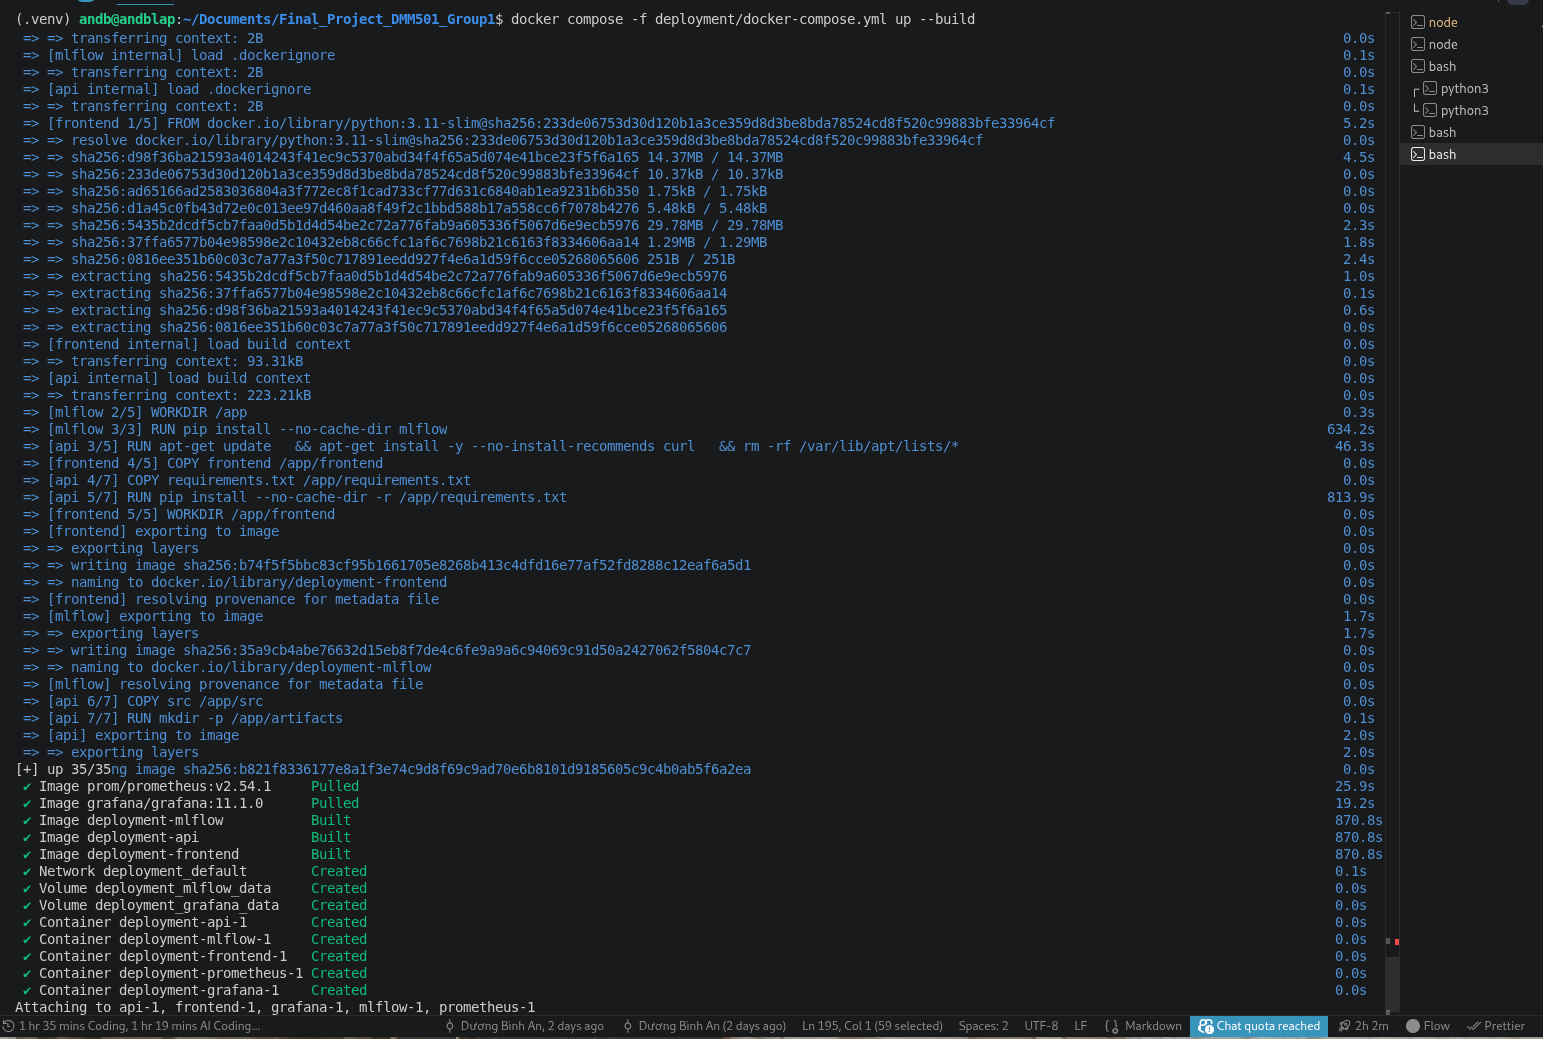
\includegraphics[width=0.95\textwidth]{docker-terminal.png}
\caption{Local \code{docker compose} up and running services (deployment evidence).}
\end{figure}

\subsection{Deployment configuration (selected environment variables)}
The deployment uses environment variables to control model selection, persistence mode, authentication, and monitoring integration. The most important variables are:

\begin{table}[H]
\centering
\begin{tabular}{p{0.32\linewidth}p{0.58\linewidth}}
\toprule
Variable & Meaning \\
\midrule
\code{MODEL\_PATH} & Path to the deployed artifact inside the API container (mounted from \code{artifacts/}). \\
\code{MODEL\_VERSION} & A human-readable identifier returned in \code{/health} and responses for traceability. \\
\code{CASE\_REPOSITORY\_MODE} & \code{memory} (demo) or \code{postgres} (durable storage). \\
\code{CASE\_DB\_URL} & SQLAlchemy connection URL for PostgreSQL when \code{postgres} is enabled. \\
\code{CASE\_DB\_AUTO\_MIGRATE} & When \code{true}, applies DB schema migrations at startup (demo convenience). \\
\code{API\_AUTH\_ENABLED} & When enabled, requires a token for protected endpoints. \\
\code{API\_TOKENS} & Token-to-role mapping used for viewer/analyst/admin authorization. \\
\code{RATE\_LIMIT\_ENABLED} & Enables request rate limiting middleware. \\
\code{MLFLOW\_RUNTIME\_ENABLED} & Enables MLflow runtime traffic tracking. \\
\code{MLFLOW\_RUNTIME\_TRACKING\_URI} & MLflow server URI used by the runtime tracker. \\
\bottomrule
\end{tabular}
\caption{Selected deployment environment variables.}
\end{table}

\subsection{CI/CD automation (GitHub Actions)}
The repository includes CI workflows for Python tests and container build validation:
\begin{itemize}
  \item \code{.github/workflows/ci.yml}: unit tests, integration tests, and a coverage gate.
  \item \code{.github/workflows/docker.yml}: Docker image builds for API and frontend, plus \code{docker compose config} validation.
\end{itemize}

\subsection{System components table}
\begin{table}[H]
\centering
\begin{tabular}{p{0.22\linewidth}p{0.2\linewidth}p{0.34\linewidth}p{0.14\linewidth}}
\toprule
Component & Role & Evidence in repository & Status \\
\midrule
Logistic regression model & Fraud scoring & \code{artifacts/models/final_model.joblib}, \code{model_info.json} & Implemented \\
Decision policy service & Map score to tier and recommendation & \code{src/services/decision_service.py} & Implemented \\
Reason code service & Produce decision-support cues & \code{src/services/reason_code_service.py} & Implemented, heuristic \\
FastAPI backend & Serve scoring and workflow APIs & \code{src/api/main.py} & Implemented \\
In-memory repository & Default alert and case storage & \code{src/repositories/in_memory_case_repository.py} & Implemented, demo-level \\
SQL/Postgres repository & Durable case storage path & \code{src/repositories/sql_case_repository.py} & Implemented (configurable) \\
Frontend dashboard & Analyst queue and case handling UI & \code{frontend/} & Implemented \\
Prometheus metrics & Operational observability & \code{src/monitoring/metrics.py} & Implemented \\
Grafana dashboards & Visualization layer & \code{deployment/grafana/} & Implemented \\
MLflow tracking & Experiment and runtime tracking & \code{deployment/mlflow/}, \code{src/monitoring/mlflow_runtime_tracker.py} & Implemented \\
\bottomrule
\end{tabular}
\caption{System components and implementation status.}
\end{table}

\section{Testing and Validation}
The repository contains unit, data, integration, security, frontend/API, SQL persistence, and model validation tests. The test inventory includes coverage for preprocessing behavior, request ID generation, dataset path handling and sampling logic, model training artifact creation, model probability range validation, key API endpoints, \code{alert} and \code{case} lifecycle flow, token-based authorization, audit events, rate limiting, SQL repository persistence across app restarts, and frontend-to-API interaction.

The repository contains unit, integration, data, model, and frontend/API tests under \code{tests/}. In the present workspace, integration-style checks pass for multiple API and workflow scenarios, but full-suite runs can encounter Windows temp-directory permission issues affecting tests that use \code{tmp_path}. This is an environment constraint rather than evidence that the implemented API workflow is absent.

\section{Responsible AI}
The repository is explicit that the system is a decision-support system and not a fully autonomous fraud adjudication engine. This is the correct framing for banking use.

Three Responsible AI points are especially important: fairness limitations because the dataset does not contain explicit protected attributes; explainability limitations because the core features are PCA-transformed and the reason codes are heuristic rather than causal; and human-in-the-loop design because final outcomes such as \code{CONFIRMED_FRAUD} and \code{FALSE_POSITIVE} are produced through \code{case} resolution, not directly by the model score.

\section{Results and Discussion}
The project demonstrates that a relatively simple model can perform well on the benchmark dataset when paired with explicit threshold policy and workflow design. The saved artifacts show strong ROC-AUC and meaningful PR-AUC, while the review and high-risk thresholds provide different operating points for queueing and containment.

The system's main strength is integration. It aligns model output, backend orchestration, frontend handling, and monitoring into a coherent fraud decision-support process. The inclusion of \code{alert} generation, \code{case} creation, status transitions, timeline events, Prometheus metrics, and Docker deployment makes the repository materially stronger than a standalone notebook or scoring endpoint.

\section{Limitations}
\begin{itemize}
  \item Dataset limitation: the Kaggle dataset is a public benchmark and does not represent the full richness of real banking transactions.
  \item PCA feature opacity: \code{V1}--\code{V28} are not business-interpretable features.
  \item In-memory persistence by default: the primary demo path stores \code{alert} and \code{case} records in process memory.
  \item Security maturity gap: token-based role checks, rate limiting, and audit events exist, but enterprise-grade IAM and hardened RBAC governance are not fully implemented.
  \item No drift detection: the repository does not implement live data drift, concept drift, or automated retraining triggers.
  \item No closed feedback loop: resolved fraud outcomes are not yet wired into a model retraining pipeline.
\end{itemize}

\section{Future Work}
\begin{itemize}
  \item Promote the SQL repository path into the default operational mode with durable database-backed \code{alert}, \code{case}, and timeline storage.
  \item Use resolved \code{case} outcomes as supervised feedback for monitoring and retraining.
  \item Add scheduled retraining, champion-challenger evaluation, and promotion controls.
  \item Monitor feature drift, score drift, queue drift, and outcome drift.
  \item Incorporate interpretable transactional features such as merchant, beneficiary, device, geography, and authentication context.
  \item Extend current token-role checks into stronger RBAC, identity integration, and hardened audit retention.
\end{itemize}

\section{Conclusion}
This repository implements a coherent real-time fraud detection system for banking-style transaction decision support. Its core contribution is the integration of machine learning scoring with operational workflow: the system computes an uncalibrated \code{risk_score}, maps it to a \code{risk_tier} and \code{decision_recommendation}, creates an \code{alert} and \code{case} for suspicious transactions, supports analyst investigation, and exposes monitoring and deployment components around that workflow.

The project therefore contributes more than a fraud model. It demonstrates how fraud analytics, backend services, frontend operations, and MLOps tooling can be combined into an end-to-end fraud decision-support system.

\section*{Implementation Status Matrix}
\addcontentsline{toc}{section}{Implementation Status Matrix}
\begin{table}[H]
\centering
\begin{tabular}{p{0.38\linewidth}p{0.16\linewidth}p{0.32\linewidth}}
\toprule
Capability & Status & Notes \\
\midrule
ML scoring API & Implemented & Artifact-backed deployed model and inference path \\
\code{risk_tier} and \code{decision_recommendation} policy & Implemented & Explicit threshold and policy mapping \\
\code{alert} and \code{case} creation & Implemented & Triggered for \code{REVIEW} and \code{HIGH} \\
Investigation timeline & Implemented & Timeline endpoint and event model present \\
Frontend analyst workflow & Implemented & Dashboard, queue, case actions, and timeline \\
Prometheus and Grafana monitoring & Implemented & Metrics, rules, and dashboard assets present \\
MLflow runtime tracking & Implemented & Runtime traffic tracker and deployment service present \\
SQL/Postgres persistence & Implemented (configurable) & Repository path, migrations, and Compose wiring are available \\
Reason-code explainability & Partially implemented & Heuristic and policy-derived rather than causal \\
Streaming behavior & Demo-level & Pull-based simulator, not event-bus-backed banking ingestion \\
In-memory case persistence & Demo-level & Process-bound storage intended for local demo \\
Enterprise RBAC/IAM and audit hardening & Future work & Current controls are token-based and limited \\
Drift detection and automated retraining & Future work & Not implemented \\
Real banking feature enrichment & Future work & Current data source is benchmark-style and anonymized \\
\bottomrule
\end{tabular}
\caption{Implementation status matrix.}
\end{table}

\end{document}
